\section{Analysis}
\label{sec:analysis}

\subsection{WF+DNS attacks}
% flow:
% - we get signal (precision), confirming what kNN says
% - signal depends on pct of exit bandwidth, but improve precision
% 	already at small pct (but big impact on recall)
% - signal depends on monitored sites' popularity

We perform 10-fold cross-validation for all of our experiments in the open
world setting. We monitor 1000 sites with 100 instances each and
$100*1000$ unmonitored sites unless otherwise stated.
\fixme{data collection}
Note the 1:1 ratio between monitored traces and unmonitored traces,
ensuring that for the classifier there is equal probability in the testing
phase that a trace is a monitored or unmonitored site.
In other words, the \emph{base rate} is 0.5 in our experiments.
Furthermore, for all experiments we specify the starting Alexa rank of the
monitored sites. Whem minitoring 1000 sites starting at rank 1, sites
[1,1000] are monitored and Alexa [1001,101000] unmonitored. Starting to monitor
Alexa from rank 100 means that Alexa sites [101,1100] are monitored, and Alexa
 [1,100] and [1101,10100] unmonitored.
We never monitor an unmonitored site or vice versa. How popular monitored sites
are is a key factor in the effectiveness of our attacks.
% note: base rate is per user, while popularity in Alexa for DNS observations
% is world-wide

Figure~\ref{fig:wfdns:torpct} shows the recall and precision for our WF+DNS
attacks as a function of the percentage of observed Tor exit bandwidth by the
attacker monitoring Alexa sites from rank $10^5$.
% TODO: consider moving recall and precision to background
Recall measures the probability that a visit to a monitored page will
be detected, while precision measures the probability that a classification by
the classifier of a visit to a monitored site (positive test outcome) is the
correct one. %Note that precision captures the base rate in an experiment.
For recall both \texttt{ctw} and \texttt{hp} are bound by the
percentage of exit bandwidth observed by the attacker (the percentage is an
upper bound).
Simply put, an attacker cannot identify a monitored site in the DNS data that
she does not see. Note that \texttt{ctw} sees improved recall over \texttt{wf}
at 100\% of exit bandwidth.
For precision our attacks have an imediate gain over \texttt{wf} as soon as
the attacker can observe \emph{any exit bandwidth}.
While the \texttt{hp} attack has constantly near-perfect precision, the
\texttt{ctw} attack benefits from observing more and more of exit bandwidth,
nearly reaching the same levels as \texttt{hp} at 100\%.


\begin{figure}[t]
\centering
\subfigure[Recall]{
	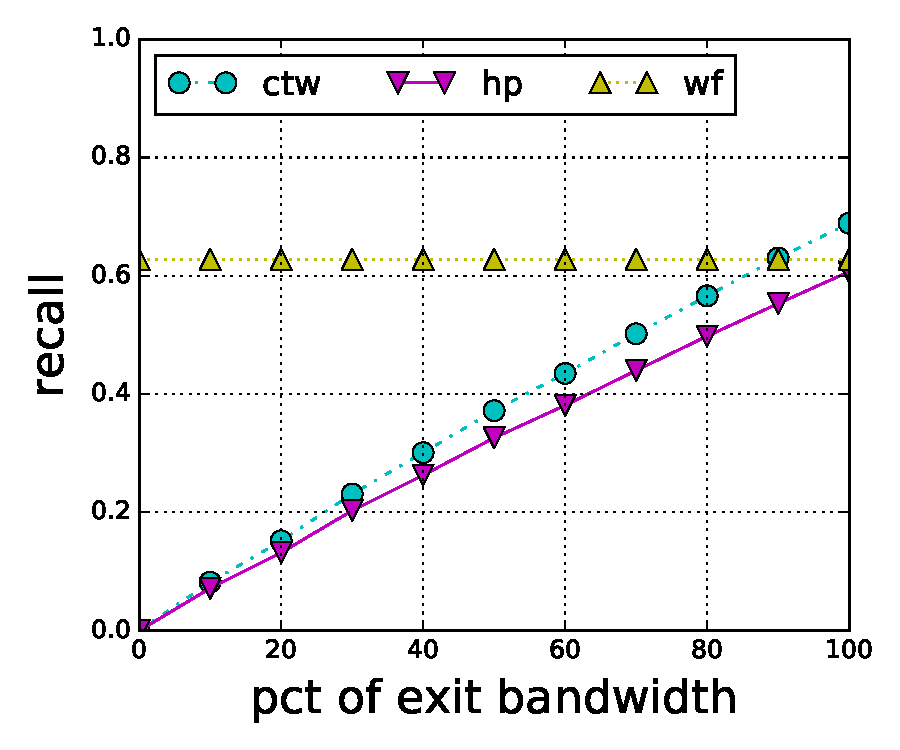
\includegraphics[width=0.466\linewidth]{figures/wfdns/pct/100x100+10000-dns2site-alexa10000-recall}
    \label{fig:wfdns:torpct:recall}
}
\subfigure[Precision]{
	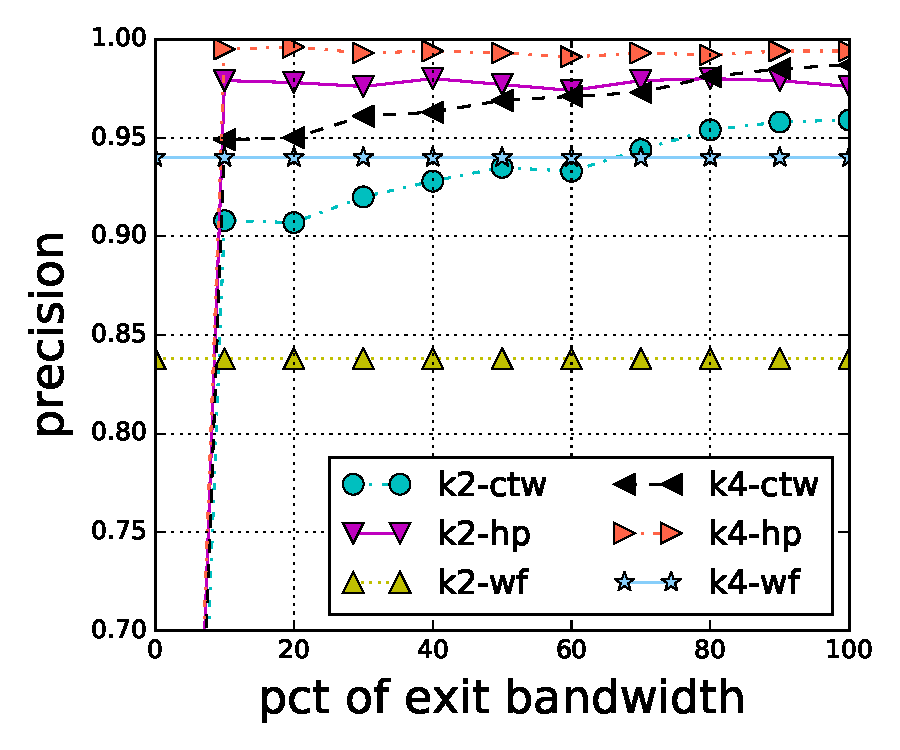
\includegraphics[width=0.466\linewidth]{figures/wfdns/pct/100x100+10000-dns2site-alexa10000-precision}
    \label{fig:wfdns:torpct:precision}
}
\caption{The recall and precision for an open-world dataset, monitoring sites
starting from Alexa rank 10k, comparing our attacks (\texttt{ctw and
 \texttt{hp}}) to a website fingerprinting attack (\texttt{wf}) for different
 percentages of observed exit bandwidth. }
\label{fig:wfdns:torpct}
\end{figure}


Figure~\ref{fig:wfdns:alexa} shows recall and precision at 100 percent of
observed Tor exit bandwidth as a function of the starting Alexa rank of
monitored sites (we still monitor 1000 sites).
For low Alexa ranks there is no difference between our attacks and the
\texttt{wf} attack. This is because, even with a window of only 60 seconds,
it is virtually guaranteed that someone browsed to any of the most popular
sites over Tor. At Alexa rank $10^3$ and onward we se a clear divergence from
the \texttt{wf} attack for both recall and precision:
\texttt{ctw} can improve the recall and precision, while
\texttt{hp} offers almost perfect precision already at Alexa $10^4$.

\begin{figure}[t]
\centering
\subfigure[Recall]{
	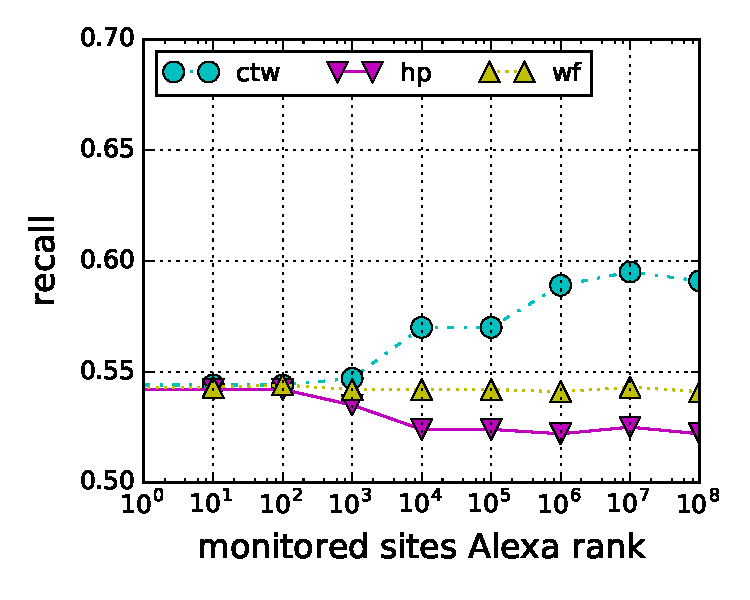
\includegraphics[width=0.466\linewidth]{figures/wfdns/alexa/1kx100+100k-offsets-100pct-recall}
    \label{fig:wfdns:alexa:recall}
}
\subfigure[Precision]{
	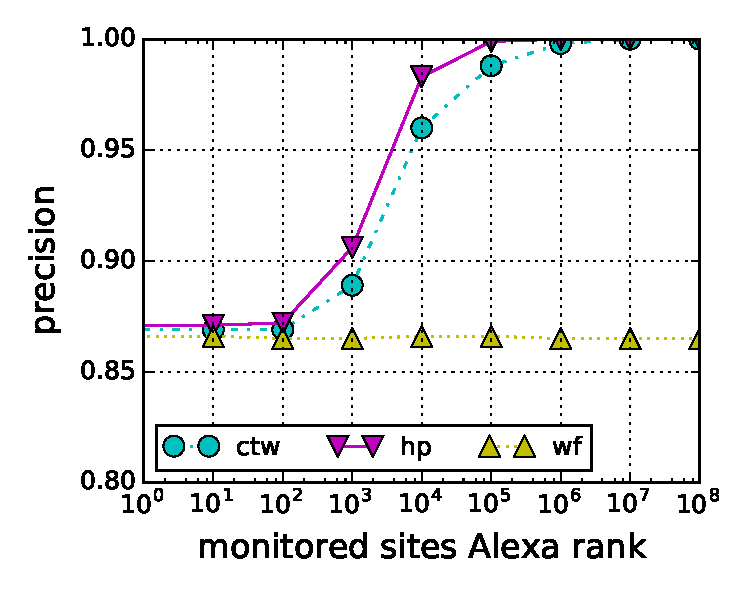
\includegraphics[width=0.466\linewidth]{figures/wfdns/alexa/1kx100+100k-offsets-100pct-precision}
    \label{fig:wfdns:alexa:precision}
}
\caption{The recall and precision when varying the starting Alexa rank of
monitored sites.}
\label{fig:wfdns:alexa}
\end{figure}

The above results paint a bleak picture: a small fraction of exit
bandwidth provides a perfectly precise attack on relatively
\emph{unpopular} sites such as \url{wikileaks.org} at Alexa rank 10808.
To better understand the limitations of our attacks, we focus on precision
and 33\% of exit bandwith (as observed on average by Google).

% window = 1800
% size = 10
% wf
% distributions


% limitation: webSITES, not wePAGES in our analysis + what we get from DNS.
